\documentclass{article}
\usepackage[top=.5in, bottom=.5in, left=.9in, right=.9in]{geometry}
\usepackage[latin1]{inputenc}
\usepackage{enumerate}
\usepackage{hyperref}
\usepackage{graphics}
\usepackage{graphicx}
\usepackage{caption}
\usepackage{subcaption}
\usepackage{tabularx}
\usepackage{amsmath}
\usepackage{amssymb}
\usepackage{siunitx}
\usepackage{mathtools}

\newcommand{\obar}[1]{\ensuremath{\overline{ #1 }}}
\newcommand{\iid}{\ensuremath{\stackrel{\textrm{iid}}{\sim}}}

\usepackage{xcolor}
\definecolor{darkgreen}{rgb}{0,0.25,0}
\newcommand{\soln}{{\color{red}\textbf{Solution:~}\color{black}}}


\usepackage[formats]{listings}
\lstdefineformat{R}{~={\( \sim \)}}
\lstset{% general command to set parameter(s)
basicstyle=\small\ttfamily, % print whole listing small
keywordstyle=\bfseries\rmfamily,
keepspaces=true,
% underlined bold black keywords
commentstyle=\color{darkgreen}, % white comments
stringstyle=\ttfamily, % typewriter type for strings
showstringspaces=false,
numbers=left, numberstyle=\tiny, stepnumber=1, numbersep=5pt, %
frame=shadowbox,
rulesepcolor=\color{black},
,columns=fullflexible,format=R
} %
\renewcommand{\ttdefault}{cmtt}
% enumerate is numbered \begin{enumerate}[(I)] is cap roman in parens
% itemize is bulleted \begin{itemize}
% subfigures:
% \begin{subfigure}[b]{0.5\textwidth} \includegraphics{asdf.jpg} \caption{} \label{subfig:asdf} \end{subfigure}
\hypersetup{colorlinks=true, urlcolor=blue, linkcolor=blue, citecolor=red}


\graphicspath{ {C:/Users/Evan/Desktop/} }
\title{\vspace{-6ex}Homework 2\vspace{-2ex}}
\author{Evan Ott \\ UT EID: eao466\vspace{-2ex}}
%\date{DATE}
\setcounter{secnumdepth}{0}
\usepackage[parfill]{parskip}



\begin{document}
\maketitle

\section{Stochastic Gradient Descent}
\subsection{(A)}
I proved this last time (see \texttt{/hw1/hw1.pdf} on GitHub), by showing
\begin{align*}
\nabla l(\beta)&=-\sum_{i=1}^N\left[y_i-m_i w_i(\beta)\right]x_i\\
w_i(\beta)&=\frac{1}{1+\exp\left(-x_i^\top \beta\right)}\\
\hat{y}_i&=m_i w_i(\beta)\\
\nabla l(\beta)&=-\sum_{i=1}^N\left[y_i-\hat{y}_i\right]x_i\\
&=\sum_{i=1}^N\left[\hat{y}_i-y_i\right]x_i\\
g_i(\beta)&=\left[\hat{y}_i-y_i\right]x_i\\
\nabla l(\beta)&=\sum_{i=1}^N g_i(\beta) ~~~~_\blacksquare
\end{align*}

\subsection{(B)}
I think all this proof needs is:
\begin{align*}
E[ng_i(\beta)] = n E_{\{x_i, y_i\} \in \{X, Y\}}[g_i(\beta)]=n \frac{1}{n}\sum_{i=1}^n g_i(\beta)=\nabla l(\beta)
\end{align*}

\subsection{(C)}
To start, I built my code on top of the functions from the first homework, looping through a fixed number of iterations,
with the following inner loop:
\begin{lstlisting}[language=R]
    ...
    pt = sample(1:N, 1)
    xSample = matrix(X[pt,], nrow = 1)
    ySample = matrix(Y[pt,], nrow = 1)
    gL = gradL(xSample, beta, ySample, m)
    beta = beta - step * gL
    ...
\end{lstlisting}
where \texttt{gradL} computes the gradient of the negative log-likelihood. This selects a point (with replacement),
computes the gradient of the log-likelihood, and uses it to update $\beta$. This way, all the rest of the code from homework 1 can be re-used.

\begin{figure}[h]
\begin{center}
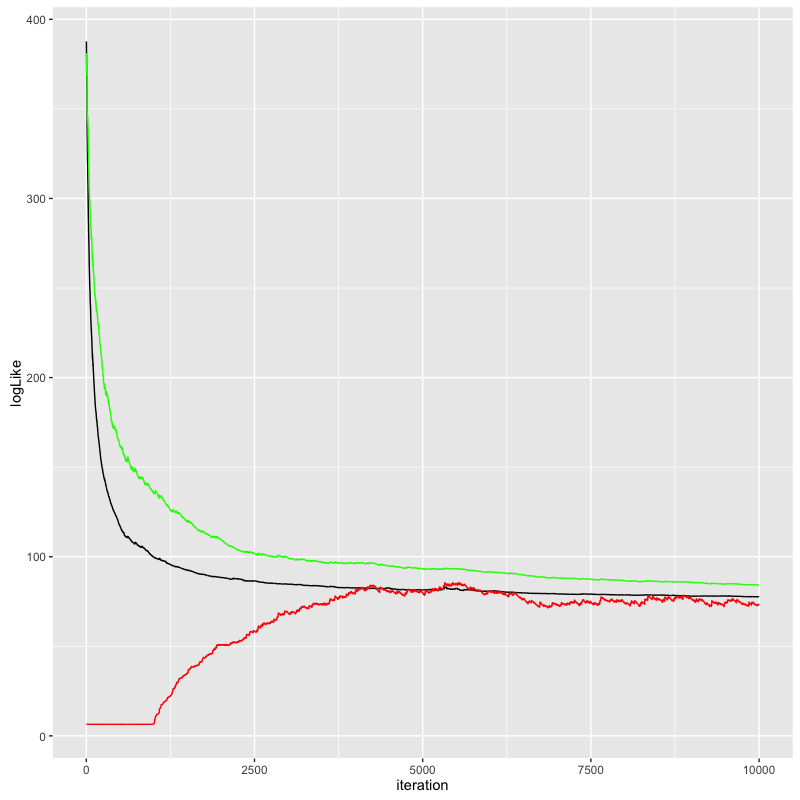
\includegraphics[scale=0.5]{partC.png}
\caption{\label{fig:c}Results for code in part C with $\gamma^{(t)}=\gamma=0.01$, 10000 iterations, and a constant of 
$\alpha=0.5 / N$ for the exponentially-weighted moving average. In black, the full negative log-likelihood, computed
on all data for reference. In green, the simple moving average. In red, the exponentially-weighted moving average.}
\end{center}
\end{figure}





\subsection{Notes from class}
The individual directions in stochastic gradient descent are like those of a drunk person telling you how to get to
NYC from Austin. Each one isn't trustworthy, but on average, they'll be decent if you take 5-mile steps. 

Essentially, the EWMA should end up being a stationary stochastic process, that is, it should bounce around a constant value. There are tests for that kind of behavior.

Having a ``memory'' in the EWMA that's too long will show really smooth progress, even potentially when the actual algorithm has converged. Too short and it'll be too noisy.


\end{document}